\documentclass[oneside, a4paper, openany]{book}

\usepackage[inner=3cm,outer=3cm,bottom=2cm]{geometry} % Sets the margins of the document
\usepackage[utf8]{inputenc}
\usepackage[british]{babel} % Use British english for hyphenation etc
\usepackage{float} %required for the placement specifier H
\usepackage{tocbibind} % Auto add Bibliography etc to Table of Contents
\usepackage{subcaption} % Creating complex figures
% \usepackage{rotating} % Used to display full page figures
\usepackage[round]{natbib} % Use BibTeX for bibliography management
\setcitestyle{notesep={: }} % Sets the cite separator to column instead of comma
\usepackage{graphicx}
\usepackage{tikz} % Inline drawing
\usetikzlibrary{decorations.pathreplacing}
\usepackage{tabu} % Easier longtables
% \usepackage{url}
\usepackage{hyperref} % Create hyperlinks within text
\usepackage[toc,nonumberlist,nopostdot]{glossaries}

\makeglossaries % Creates the glossary section

\graphicspath{{./assets/}{./assets/wireframe/}{./assets/design/}}
\begin{document}

\frontmatter
\begin{titlepage}
  \newcommand{\HRule}{\rule{\linewidth}{0.5mm}}
  \center

  \textsc{\LARGE Robert Gordon University}\\[1.5cm]
  \textsc{\Large Bachelor of Science in Computer Graphics and Animation}\\[0.5cm]
  \textsc{\large Honours Project Report}\\[0.5cm]

  \HRule \\[0.4cm]
  { \huge \bfseries A Mobile Application that applies Self-Management Approach to Reduce Sedentary Behaviour}\\[0.4cm]
  \HRule \\[1.5cm]

  \begin{minipage}{0.4\textwidth}
  \begin{flushleft} \large
  \emph{Author:}\\
  Georgi \textsc{Koemdzhiev}
  \end{flushleft}
  \end{minipage}
  ~
  \begin{minipage}{0.4\textwidth}
  \begin{flushright} \large
  \emph{Supervisor:} \\
  Dr. Stewart \textsc{Massie}
  \end{flushright}
  \end{minipage}\\[4cm]

  {\large 2017}\\[3cm]

  \includegraphics[width=5cm, scale=0.1]{rgu-logo.png}\\[1cm]
  \vfill
\end{titlepage}
\chapter{Declaration}
I confirm that the work contained in this Honours project report has been composed solely by myself and has not been accepted in any previous application for a degree. All sources of information have been specifically acknowledged and all verbatim extracts are distinguished by quotation marks.\\[2cm]

  \noindent Georgi Koemdzhiev\\
  5th December 2016
\chapter{Abstract}
Sedentary behaviour is a leading cause of numerous chronic deceases, but currently, there is a lack of mobile applications that try to help tackle this problem. The purpose of this paper is to show how behaviour change techniques can be applied in a mobile application to help people change their sedentary habits. This project proposes a smartphone application that uses daily activity guidelines to increase physical activity. This software will be developed based on findings from background research. It will incorporate behaviour change techniques that will allow maintaining a good goal-performance relationship. Also, self-management logic will be present to facilitate self-care features such as setting a psychical activity goal.
\chapter{Acknowledgements}
Firstly, I would like to express my gratitude to my supervisor Dr Stewart Massie of Robert Gordon University for his guidance during the research and development of the project. \\

\noindent Besides my supervisor, I would like to thank the designers and developers at xDesign for sharing their knowledge and experience with me; my parents Vangel Koemdzhiev and Violeta Koemdzhieva for encouragement me throughout writing this thesis and my partner Mariya Menova for her support and understanding.

% \setcounter{tocdepth}{4}
\tableofcontents
\input{frontmatter/list-of-figures}
\input{frontmatter/list-of-tables}

\newglossaryentry{har}
{
  name=HAR,
  description = {Human Activity Recognition}
}

\newglossaryentry{gsc}
{
    name=GSC,
    description = {Goal-Setting Component}
}

\newglossaryentry{mc}
{
    name=MC,
    description = {Monitoring Component}
}

\newglossaryentry{fc}
{
    name=FC,
    description = {Feedback Component}
}


\glsaddall %Print all entries %
\setglossarystyle{altlist}
\printglossaries

\mainmatter
\chapter{Introduction}
\label{Chapter:Introduction}
Nowadays, with the rapid advance of technology people spend a lot of their time in a static position. According to \citet{wilmot2012} that increases the chances of all-cause mortality by 49\%.  Also, people who lead non-active lifestyle are 112\% more likely to get diabetes, 147\% more likely to experience cardiovascular events, and 90\% more likely to die due to cardiovascular events. 
    
Using self-manageing systems to counter sedentary behaviour is becoming a well-accepted solution due to its many advantages over the traditional paper based methods. This paper proposes a self-management mobile application that apples behaviour change logic to reduce sedentary time as well encourage more physical activity. 
    
    \section{Project Catalyst}
    My passion for software began back in my first year as a student at Robert Gordon University. I was exposed to various modules related to software development which I found absorbing. Consequently, I was able to do a summer internship with a company called xDesign as a Software Engineer and thus gain industry knowledge and skills. I was confident that mobile application development was an area I wanted to pursue. 
    
    This passion for software contributed immensely on the topic of my honours project. Also, the idea of the health aspect of the mobile application made the subject even more appealing to me. My application could potentially help people self-manage their sedentary time as well as promote more physical activity. 
    
    
    \section{Goals and Objectives}
    A set of goals and objectives were formed prior to the initiation of the project to help shape its scope. The goals of the project define the main motivation behind it whereas the objectives underline the main tasks that the project undertakes.
    
    \subsection*{Goals}
    The following project goals have been identified: 
    \begin{enumerate}
        \item Satisfy the requirements the of BSc (Hons) Computing (Graphics and Animation) course
        \item Demonstrate future employers programing as well as UI/UX design skills
        \item Gain a better understanding of how machine learning works 
        \item Go through the main stages of the software development process
    \end{enumerate}
    
    \subsection*{Objectives}
    The following list of objectives helped accomplishing the above goals: 
    \begin{enumerate}
        \item Gather information about Self-Management in the Health sector
        \item Research Sedentary Behaviour factors and consequences
        \item Research behaviour change methods
        \item Research how to implement Human Activity Recognition 
        \item Design and Implement a mobile application on the Android platform based on the project research findings
    \end{enumerate}
    
    \section{Document structure}
    This section of the document addresses how this report is organised.\newline
    
    \textbf{Literature Review} Gives a wide background information regarding using self-management technologies in the health sector, Behaviour changing techniques, consequences and current situation of of Sedentary Behaviour as well as researching commercial and non-commercial HAR mobile applications.\newline
    
    
    \textbf{Specification} Lists the proposed mobile application Functional and Non-functional requirements as well as discussing the system quality attributes. The information in this chapter is heavily influenced by the \textit{Literature Review} chapter.\newline
    
    
    \textbf{Design} Addresses the system design decisions\newline
    
    
    \textbf{Implementation} Details about how the system design have been implemented for each of the main system components.\newline
    
    
    \textbf{Evaluation} A discussing how effective is the implemented system on users.\newline
    
    
    \textbf{Conclusion} Summary of the potential benefits of Sedentary Behaviour self-manageing devices in the health sector, future work and project critical appraisal.\newline
    
    
    \section{Professional, Social, Ethical, Security and legal issues to the project}
    
    \subsection{Professional}
    As a student studying Computing for Graphics and Animations – a course that is accredited by the British Computer Society (BCS) I intend to comply with the BCS Code of Conduct. Specifically point 4 (d) \citep{bcs_2017} - “act with integrity and respect in your professional relationships with all members of BCS…” I intend to acknowledge the authors of any third party software use in this project.

    \subsection{Social}
    The proposed application will try to avoid promoting any body image stereotypes by focusing more on encouraging the users to be more active rather than on their body characteristics such as weight and height or BMI (Body Mass Index). In addition, the application will only show what the recommended activity intervals per day are and will not force the users of the application to follow those strictly (some jobs do require seating for extended intervals of time – e.g. Pilots).
    
    \subsection{Ethical}
    The data collected during the project development such as names of the project participants and their accelerometer sensor data will be stored on disk only for the development purposes of the project. 
    
    \subsection{Security}
    The mobile application, proposed in this work, will offer an authorisation component to prevent other people accessing personal data such as total minutes of activity/inactivity collected daily. What is more, any relevant or valuable user data will be anonymised to protect individual’s identity.

    
    \subsection{Legal}
    To prevent any harm done to the user, the mobile application will show a disclaimer (warning) dialog message to inform the user that they should be in a good physical condition (not suffering from diseases that could lead to worsening the condition of the user) before they use the application. In addition, I intend to fully comply with the terms of conditions of any third party software that I intend to use (my main goal is to use primarily Open Source software). As far as the project participant’s data is concerned, I intend to keep the data only for the purposes of this project, and the data will not be used for any commercial purpose. 

\chapter{Literature Review}
\label{Chapter:Literature-Review}

As it was mentioned in Chapter \ref{Chapter:Introduction} this document proposes a system implemented on a mobile device that encourages the reduction of sedentary time via self-management techniques. In order to gain knowledge on how to devise such as system, literature review needs to be carried away on several topics. First of all, the current shift towards self-management in the health sector will be discussed. The next section will focus on evaluating how much time people spend in Sedentary Behaviour (SB) and what are the consequences. Section 3 looks at digital behaviour change techniques. Commercial and non-commercial \gls{har} mobile applications and \gls{har} itself are discussed in Section 4. Section 5 summarises the system proposed.

\section{Self-Management in the Health Sector}
 \label{section:sm-in-hs}
    Mobile devices with embedded self-management logic are currently being utilised and becoming a well-accepted solution for millions of people in the health sector. For example, the NHS’s England Executive – Simon Stevens, launched a programme “Test Beds” \citep{nhsengland2016,nhsengland2016a} which is a set of collaborative projects between NHS and some technology companies such as Verily, IBM and Philips. The idea behind the project is to test the effectiveness of different technological innovations, including wearable devices and mobile applications. These technologies will enable patients to self-manage illnesses such as diabetes, heart diseases and dementia.
    
    \subsection{Advantages of self-management}
    Shifting towards self-care via mobile devices has many advantages over the traditional methods (e.g., over the phone or face-to-face). For example, self-care devices enable patients to monitor their illnesses at home. \citet[10]{roberts2006} finds that patients using wearables improve their condition and shorten their recovery time if they can be in a familiar environment. Real-time feedback is another advantage of using self-management devices. For example, \citet{alivecor2016}, can prevent critical and even fatal incidents by identifying illness clues ahead of time. Thus, the number of patients becoming seriously ill or needing hospital treatment will potentially be reduced. Consequently, that could save money on hospital treatments \citep{campbell2016}. In addition, \citet[6]{shuger2011} found that real-time feedback on \gls{sb} could be beneficial for weight loss. \citet[97]{whitehead2016} concludes that self-management approaches delivered via mobile applications have the potential to improve outcomes of many chronic diseases.
    
    \subsection{Need for self-management devices}
    It has been found that there is a gap in the current market regarding self-care devices that focus on monitoring \gls{sb} and not only \gls{pa}. For example, \citet{sanders2016} found out that there is a lack of self-management mobile applications or devices on the market that can monitor \gls{pa}. After research, he was able to find 73 devices that provide self-monitoring of PA, and only 9 can monitor sedentary time (see Figure \ref{fig:devices-to-provide-SB-feedback}). That means that there is a lack of products in the market that offer self-management of SB in addition to PA. Sanders also concluded that the current devices capable of measuring sedentary time and providing feedback have not been used in behaviour change interventions. In conclusion, there is a need for further research and development of self-care enabled wearables to help people engage in behaviour change interventions and prevent possible chronic diseases. 
    
    \begin{figure}[h]
        \centering
        \includegraphics[width=10cm]{figureOne}
        \caption{Current technologies that self-monitor and provide feedback on SB \citep{sanders2016}}
        \label{fig:devices-to-provide-SB-feedback}
    \end{figure}

\section{Sedentary Behaviour}

Understanding the consequences of \gls{sb} as well as recommended daily energy expenditure levels is crucial for developing a mobile application that aims to implement behaviour changing theory. It is said that there is a difference between \gls{sb} and \gls{pa} and these terms should be treated differently \citep[540]{networ2012}. For example, a person can do both be sedentary for prolonged periods of time and spend large amounts of vigorous physical activity in one day. Networ define \gls{sb} as “energy expenditure less or equal to 1.5 METs while in a sitting or reclining posture” (see Table 1 for comparison of different activities). As it can be seen from Table \ref{fig:activity-intensities}, the energy spent in static activities does not result in a lot of energy expenditure and that potentially could lead to the occurrence of chronic diseases. \citet[540]{networ2012} also defines a person who is “inactive” as “not meeting specified physical activity guidelines”. That means that a person has to meet the PA recommendation levels in order to be considered as active. The next section will discuss the consequences of SB and the suggested amount of physical activity per day.

    \begin{figure}[h]
        \centering
        \includegraphics[width=10cm]{tableOne}
        \caption{Examples of light, moderate, and vigorous activities \citep{harvardthchanschoolofpublichealth2012}}
        \label{fig:activity-intensities}
    \end{figure}
    
    \subsection{SB consequences and PA recommendations}
    Sedentary Behaviour has been positively associated with diseases such as back pain, diabetes, cardiovascular disease, cancer and all-cause mortality (Wilmot et al., 2012: 2895–2905, Biswas et al., 2015: 123 and Department of Health, 2010: 18). In addition, Biswas et al. (2015: 127) even concluded that SB causes adverse outcomes regardless of the physical activity, although the chances of developing a SB associated chronic diseases are low when involved in higher levels of physical activity.
    
    As far as the PA recommendations are concerned, the Department of Health (2011) and Townsend et al. advocate for 30 minutes of PA for every day of the week. What is more, Parkinson (2016) and Siddique (2016) state that an ideal PA per day would be an hour. Having said that, simply doing 30 minutes or even an hour of activity is not enough. For example, a person may do 30 minutes of activity a day and spend the rest of the time laying or sleeping. To counter that, Swartz, Squires, and Strath (2011) suggest that every static hour should be interrupted by at least of a five-minute walk.
    
    \subsection{Current statistics of sedentary behaviour}
    \citet[19]{townsend2015} found in 2012 that 34\% of adult man and 46\% of adult women did not meet the recommended levels of physical activity. Also, according to \citet[81]{townsend2015}, 45\% of the adults in the UK spend up to 5h and 30 minutes in SB such as watching TV, using a computer or playing video games. What is more, \citet{swinford2014} found in a survey that there has been an increase in the time people spend in sedentary activities compared to 1995. For example, he found that people nowadays take 18 per cent fewer journeys, 24 per cent fewer go to do shopping and 28 per cent visit friends compared to 1995. In conclusion, to improve the state of the people who are spending too much time in sedentary behaviour, there is a need for further research on the effectiveness of behaviour change interventions only focusing on sedentary time and physical activity alone \citep[130]{biswas2015}.

\chapter{Specification}
\label{Chapter:Specification}

The specification of the mobile self-management application can be split into three components: Goal-setting, Monitoring and Feedback. The Goal-Setting Component (GSC), as the name implies, handles setting goals as well as providing additional information such as recommended amounts of physical activity per day. The Monitoring Component (MC) is the most complex part of the system. It is essentially a \gls{har} system with additional logic for recognising the current activity of the user (e.g. walking or static) and logging the data into a database. In addition, this component is responsible for detecting sedentary behaviour and measuring physical activity amounts. As far as the Feedback Component (FC) is concerned, it provides feedback to the user in the form of notifications. 
\section{Functional Requirements}

    \subsection{Goal-Setting Component}
    As it was mentioned in Chapter \ref{Chapter:Literature-Review},  goal-setting is an important part of the behaviour change process. It allows the user to set goals which is the first step towards better lifestyle. This component's requirements are mainly derived from the background research. 
    
    \begin{enumerate}
        \item \gls{gsc} shall allow the user to set \gls{pa} goals
        \begin{enumerate}
            \item \gls{gsc} shall provide list of recommended \gls{pa} goals
            \item \gls{gsc} shall allow the user to set custom \gls{pa} goals
        \end{enumerate}
        \item \gls{gsc} shall allow the user to set Sedentary Time (\gls{st}) goals
        \begin{enumerate}
            \item \gls{gsc} shall allow the user to set the maximum duration of \gls{st} before a reminding notification is sent 
        \end{enumerate}
    \end{enumerate}
    
    
    \subsection{Monitoring component}
    The main purpose of the \gls{mc} is to continuously recognise activities and analyse the levels of \gls{pa} and \gls{st}. The following requirements have been derived from analysing past and current mobile devices and applications.
    
    \begin{enumerate}
        \item The \gls{mc} component shall classify physical activities
        \begin{enumerate}
            \item HAR component shall recognise the following activities:
            \begin{enumerate}
                \item walking
                \item running
                \item cycling
                \item static
            \end{enumerate}
        \end{enumerate}
        \item The \gls{mc} component shall analyse user's \gls{pa} and \gls{st} amounts in real time
            \begin{enumerate}
                \item \gls{mc} shall increment user's \gls{pa} or \gls{st} value whenever physical activity or sedentary behaviour is recognised
            \end{enumerate}
        \item The \gls{mc} shall personalise \gls{har}'s classifier
            \begin{enumerate}
                \item When enough user data is collected, the system shall retrain the classifier with user's own data
            \end{enumerate}
            
        \item \gls{mc} shall keep history of previously accumulated \gls{pa} and \gls{st} amounts
        
        \item The user shall be able to set "Sleeping Hours", time interval during which no measurement of \gls{pa} or \gls{st} should occur
      
    \end{enumerate}
    
    \subsection{Feedback Component}
    The \gls{fc} is responsible for sending notifications to the user. It can provide important information such as when a previously set goal is attained or reminder for the user that they are spending too much static time.
    \begin{enumerate}
        \item \gls{fc} shall notify the user when they are being sedentary for too long (e.g. an hour)
        
        \item \gls{fc} shall notify the user when a previously set goal is attained (e.g. being active for 30 minutes)
        
        \item \gls{fc} shall not send notifications during "Sleeping Hours" time interval
    \end{enumerate}

\section{Non-functional Requirements}
The mobile application proposed in this work has to comply to a number of additional requirements. Since the \gls{gsc},\gls{mc} and \gls{fc} are all part of the same software, their non-functional requirements will be discussed all together.
    
    % \subsection{Limitations}
    
    \subsection{Accuracy}
    The accuracy of the system shall be high so that misclassification of activities are avoided or minimised. For example, classifying "walking" as "static" would lead to incorrect \gls{pa} daily readings. Consequently, the user may be doing less physical activity if they are notified they attained a goal.
    
    \subsection{Battery consumption}
    Since the resources of every portable device (i.e. mobile phone) are constrained, the system shall be designed so that it consumes reasonable amount of battery power. For example, the user must not need to charge the device in the middle of the day since that renders measuring component of the application useless (the application cannot measure \gls{pa} when the device is on the user).
    
    \subsection{Security}
    The mobile application shall store user data only on the system in order to minimise the risk of data breach. In addition, the following considerations have been taken into account:
    
    \begin{enumerate}
        \item The system shall provide protection of user's data
            \begin{enumerate}
                \item The system shall show authentication screen before showing any sensitive data
                \item The system shall encrypt the data stored in a local database
            \end{enumerate}
    \end{enumerate}
    
    \subsection{System Quality Attributes}
        
        \subsubsection{Adaptability}
        Modern mobile applications should be able to quickly adapt to new requirements as the market always changes. That is why the system design implements the \gls{mvp} software pattern which increases the ability of the system to incorporate new features easily.
        
        \subsubsection{Scalability}
        It is difficult to envision how much data will be gathered from the sensors of the smartphone. However, the system should be scalable and thus capable of handling large amounts of computations.
        
        \subsubsection{Modularity}
        The system is comprised of different units. For example, each screen is encapsulated in a separate directory which can be interchanged easily without changing the integrity of the system.  
        
        \subsubsection{Testability}
        To assure that the system works as intended, the system shall be tested by both assertions and Quality Assurance tests. 
        
        \subsubsection{Maintainability}
        The system shall be designed in such a way so that it allows for easy debugging and evolution. For example, extending the system by adding new features.
        
        \subsubsection{Robustness}
        The system will constantly work in the background (e.g. collect contextual data) so ensuring that the system encompass as many points of failure as possible is crucial.
    
    
    
\chapter{Design}
\label{Chapter:Design}

This chapter discusses the design considerations taken during the design development of the system. The design stage is very important since it lays down the foundation for the whole system. If not done right it could lead to undesired consequences later on in the implementation stage and even in the end-product. \citet[12]{bell2005} states that about 5\% of the total time that takes for the development of a software should be spent for the design state alone. For comparison, the coding takes about 7\% and Testing takes 8\%. Thus a considerable amount of time has been spent in designing the system. 

The design process has gone through many iterations to ensure the best possible quality of the product. The design can be split into two main sections, namely User Interface (UI) Design and System Architecture (SA) design.
\chapter{Development Methodologies}
\label{chapter:development_methodologies}
This chapter discuses the development practices that are used during the development process of the proposed system.  

\section{Development Model}
\label{section:development-model}
As with every software product, specific rules are needed to ensure that the software is developed in a manner that satisfy its specifications and achieves the end-goals. In the IT industry that is achieved by following a software development model. It specifies the required stages of the development and the order in which the they are carried out. In this project the \textit{Incremental Model} has been chosen to drive the development of the software. The main idea behind this model is developing a system through iterative steps and in small incremental portions \citep[264]{bhuvaneswari2013}. It ensures that each iteration (e.g. software build) is tested and working before using the previous iteration as a bases for the next one (see figure \ref{fig:incremental-model}). The The main benefits of using this model are:

\begin{itemize}
    \item A product is produced early in the project's development
    \item Because of the previous point, unforeseen problems can be detected early
    \item Client change requests can be implemented between increments
\end{itemize}

    \begin{figure}[H]
        \centering
        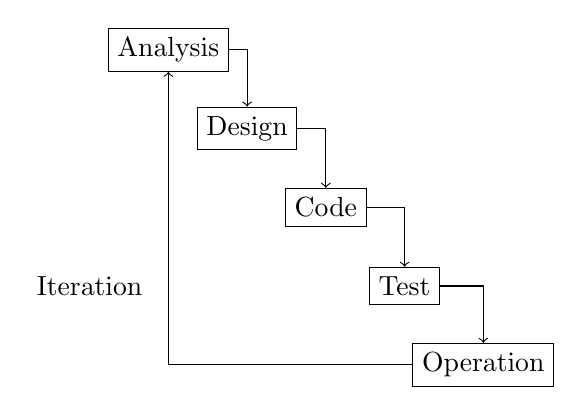
\begin{tikzpicture}
            % nodes
            \node (a1) [draw]  {Analysis};
            \node (d1) [draw, below of=a1, right of=a1] {Design};
            \node (c1) [draw, below of=d1, right of=d1] {Code};
            \node (t1) [draw, below of=c1, right of=c1] {Test};
            \node (o1) [draw, below of=t1, right of=t1] {Operation};
            \node at (-1,-3) {Iteration};
            % arrows
            \draw[->, to path={-| (\tikztotarget)}](a1) edge (d1) (d1) edge (c1) (c1) edge (t1) (t1) edge (o1) (o1) edge (a1);
        \end{tikzpicture}
        \caption{Incremental software development model life cycle}
        \label{fig:incremental-model}
    \end{figure}


\section{Version Control System}
When developing a software challenges can occur unexpectedly and a developer has to do whatever possible to ensure the their work is protected. For example, untraceable bug can be introduced in one of the iterations of the iterative development model (see section \ref{section:development-model}) that could lead to poor system performance. In order to prevent the (or at least dramatically lower)the occurrence these situations the use of \textit{"Version Control"} is encouraged.

There are many Version Control Systems (VCS) out there such as Mercurial, Fossil and Git. The main purpose of a \gls{vcs} is to keep track of the changes in a project. If a developer is satisfied with a specific change, they can perform a \textit{commit}. That action will merge the change to the codebase and the commit command will be added to the changelog (list of commits). If there is a problem that has been caused by a previous \textit{"bad"} commit, the developer can simply revert the whole project to a more stable state by restoring the codebase to a previous known \textit{"good"} commit.

For this project, Git has been chosen along with its web service GitHub\footnote{\url{https://github.com}} to serve as a \gls{vcs} due to the fact that it is easy to use and it is well-documented.


\section{Project Management}
It is important to stay organised when it comes to working on a project, especially when it involves the usage of limited resources (i.e. Time). Thus, a project management tool called \textit{Taiga.io}\footnote{\url{https://taiga.io}} was utilised to help keep track of the project's progress via \textbf{\textit{Kanban} boards}. With every incremental iteration (see \ref{fig:incremental-model} above) new tasks are identified, created and added to the Kanban boards.

Using \textit{Kanban} boards introduces several benefits to the development of the project. Firstly, it provides a quick way to organise the project work visually. For example, boards titled \textit{"READY"} and \textit{"IN PROGRESS"} tables contain that tasks that are already implemented and what those that are being implemented, respectively (see figure \ref{fig:taiga-kanban-boards}). Secondly, it increases the development efficiency since one of the key aspects of the Kanban methodology is to limit the work in progress (WIP) by setting a limit \citep[]{atlassian2017}. For example, if the number of tasks in \textit{IN-PROGRESS} board is 1, that means that no other tasks should be started until the currently undergoing one is finished.

\begin{figure}[ht]
    \centering
    \includegraphics[width=15cm]{taiga-kanban-boards}
    \caption{Taiga Kanban boards}
    \label{fig:taiga-kanban-boards}
\end{figure}

\section{MVP and Dependency Injection}
    As discussed before, the implementation of the mobile application is following the \gls{mvp} software pattern, which allows for the clear separation of code concepts (see section \ref{section:architectural-design}). To better satisfy the requirements discussed in section \ref{section:system-quality-attributes}, \gls{mvp} is combined with a Dependency Injection (DI) principle. What \gls{di} do is shifting the responsibility of one class to create its dependencies to another class. For example, class Car requires class Engine as a parameter. Instead of creating a new instance of class Engine when class Car is created it is simply provided as a constructor parameter in class Car's constructor (see listing \ref{di-car-example}).
    
     \begin{wrapfigure}{RI}{0.3\textwidth}
        \begin{center}
            \includegraphics[width=0.3\textwidth]{app-directory-structure}
        \end{center}
    \caption{Data collection screen directory structure}
    \label{fig:app-directory-structure}
    \end{wrapfigure}
    
    Dagger\footnote{\url{https://github.com/google/dagger}} is a framework that utilises the \gls{di} principle in the form of \textit{Component} and \textit{Module} classes. A module creates the necessary dependencies (e.g. object of class B) whereas the Component class determines where those dependencies will be "injected" (e.g. satisfy dependence's in class A). A concrete example of \gls{di} can be seen in Listing \ref{di-example}. In this example, the \textbf{LoginFragment} (e.g. the login screen) requires an object of type \textit{\textbf{"ILoginPresenter"}} to function. The method \textit{\textbf{"satisfyDependencies()"}} provides the dependencies to the class (e.g. externally). All of the dependencies of the Login screen are provided from a Dagger module named \textit{\textbf{"AuthModule"}} which is responsible for providing and creating the concrete implementation of the above interface (e.g. ILoginPresenter). The full code of \textit{\textbf{"AuthModule"}} as well as \textit{\textbf{"AuthComponent"}} can be seen in Appendix \ref{chapter:dagger-component-module}.  
    
        
    Combining the \gls{mvp} design pattern with dependency injection framework such as Dagger brings a lot of advantages for the software product. Firstly, the software becomes more loosely coupled as the \gls{mvp} enforces the use of interfaces and Dagger is responsible for injecting the concrete implementation of those interfaces where required. Secondly, it allows for logically structuring the codebase. For example, a common approach when using both \gls{mvp} and Dagger is to create a directory for each one of the mobile screens (see figure \ref{fig:app-directory-structure}) containing the necessary \gls{mvp} classes such as \textit{\textbf{Presenter}} and \textit{\textbf{Model}} and the as well as Dagger's \textit{\textbf{Module}} and \textit{\textbf{Component}} to handle the \gls{di} process.
    
\begin{lstlisting}[caption= DI example, label=di-car-example,frame=tlrbr,basicstyle=\small,captionpos=b]
    class Car{
        Engine engine;
            Car(Engine engine){
                this.engine = engine;
            }
       }
    }
\end{lstlisting}


\appendix
% Add more here
\chapter{Use cases}
\label{use_cases}
\section*{Log in}
    The user opens the application. The system shows the log-in screen. The user types in their username and password. If the provided credentials are valid, the system shows the main screen of the application.
    
\section*{Sign up}
    The user opens the application and go to the Sign-up screen. The system shows the Sign-up screen and opening the virtual keyboard awaiting user input. The user enters their username and password. The system verifies that the entered information is correct and creates a new user account. The user is taken to the main screen of the application.
    
\section*{Set \gls{pa} goal}
    The user opens the application. The system takes the user to the main screen. The user opens the navigation drawer and selects the \textit{Settings} menu item. The system opens the Settings screen. The user selects the "Physical Activity goal" settings item. The system shows a dialog window with list of options. The user selects the desired option. The system accepts the user input and updates the system accordingly.

\section*{Change \gls{sb} remind interval}
    The user opens the application. The system takes the user to the main screen. The user opens the navigation drawer and selects the \textit{Settings} menu item. The system opens the Settings screen. The user selects the "\textit{Notify inactivity}" settings item. The system shows a dialog window providing list of options. The user selects the remind interval and confirms their choice by pressing the "OK" button. The system accepts the user input and updates the system accordingly. 
    
\section*{Change \textit{"Sleeping Hours"}}
    The user opens the application. The system opens the main screen. The user opens the navigation drawer and selects the \textit{Settings} menu item. The system opens the Settings screen. The user selects the "\textit{Sleeping Hours}" settings item. The system shows a date picker dialog. The user selects the preferred time interval and confirms their choice by pressing the "OK" button. The system accepts the user input and updates the system accordingly.
    
\section*{Check goal progress}
    The user opens the application. The system opens the main screen (i.e. \textit{Today} screen). The user sees the amount of \gls{pa} in minutes as well as the previously set goal. The user closes the application.
    
\section*{Check activity history}
    The user opens the application. The system shows the main screen. The user opens the navigation drawer and selects the \textit{"History"} settings item. The system opens the History screen. The user sees the history of activities softed either \textit{"Daily"} or \textit{"Weekly"}. The user closes the application. 
\chapter{Screen Wireframes}
\label{chapter:screen-wireframes}

\begin{figure*}[ht]
    \centering
    \begin{subfigure}[t]{0.4\textwidth}
        \centering
        \includegraphics[width=5cm,keepaspectratio]{navigation-drawer-open}
        \caption{Navigation Drawer opened}
    \end{subfigure}%
    ~ 
    \begin{subfigure}[t]{0.4\textwidth}
        \centering
        \includegraphics[width=5cm,keepaspectratio]{today-screen}
        \caption{Main Screen}
    \end{subfigure}
    \caption{Main Screen. Navigation drawer opened.}
\end{figure*}



\begin{figure*}[ht]
    \centering
    \begin{subfigure}[t]{0.4\textwidth}
        \centering
        \includegraphics[width=5cm, keepaspectratio]{history-screen-daily}
        \caption{History Screen, mode daily}
    \end{subfigure}%
    ~ 
    \begin{subfigure}[t]{0.4\textwidth}
        \centering
        \includegraphics[width=5cm,keepaspectratio]{history-screen-weekly}
        \caption{History Screen, mode weekly}
    \end{subfigure}
    \caption{History Screens}
\end{figure*}



\begin{figure*}[ht]
    \centering
    \begin{subfigure}[t]{0.4\textwidth}
        \centering
        \includegraphics[width=5cm,keepaspectratio]{log-in-screen}
        \caption{Login Screen}
    \end{subfigure}%
    ~ 
    \begin{subfigure}[t]{0.4\textwidth}
        \centering
        \includegraphics[width=5cm,keepaspectratio]{sign-up-screen}
        \caption{Signup Screen}
    \end{subfigure}
    \caption{Authentication Screens}
\end{figure*}



\begin{figure*}[ht]
    \centering
    \begin{subfigure}[t]{0.4\textwidth}
        \centering
        \includegraphics[width=5cm,keepaspectratio]{data-collection-screen}
        \caption{Data Collection Screen}
    \end{subfigure}%
    ~ 
    \begin{subfigure}[t]{0.4\textwidth}
        \centering
        \includegraphics[width=5cm,keepaspectratio]{settings-screen}
        \caption{Settings Screen}
    \end{subfigure}
    \caption{Utility Screens}
\end{figure*}
\chapter{Screen Designs}
\label{chapter:screen-design}

\begin{figure*}[ht]
    \centering
    \begin{subfigure}[t]{0.4\textwidth}
        \centering
        \includegraphics[width=5cm,keepaspectratio]{navigation-drawer-open-design}
        \caption{Navigation Drawer opened}
    \end{subfigure}%
    ~ 
    \begin{subfigure}[t]{0.4\textwidth}
        \centering
        \includegraphics[width=5cm,keepaspectratio]{today-screen-design}
        \caption{Main Screen}
    \end{subfigure}
    \caption{Main Screen. Navigation drawer opened.}
\end{figure*}



\begin{figure*}[ht]
    \centering
    \begin{subfigure}[t]{0.4\textwidth}
        \centering
        \includegraphics[width=5cm, keepaspectratio]{history-screen-daily-design}
        \caption{History Screen, mode daily}
    \end{subfigure}%
    ~ 
    \begin{subfigure}[t]{0.4\textwidth}
        \centering
        \includegraphics[width=5cm,keepaspectratio]{history-screen-weekly-design}
        \caption{History Screen, mode weekly}
    \end{subfigure}
    \caption{History Screens}
\end{figure*}



\begin{figure*}[ht]
    \centering
    \begin{subfigure}[t]{0.4\textwidth}
        \centering
        \includegraphics[width=5cm,keepaspectratio]{log-in-screen-design}
        \caption{Login Screen}
    \end{subfigure}%
    ~ 
    \begin{subfigure}[t]{0.4\textwidth}
        \centering
        \includegraphics[width=5cm,keepaspectratio]{sign-up-screen-design}
        \caption{Signup Screen}
    \end{subfigure}
    \caption{Authentication Screens}
\end{figure*}



\begin{figure*}[ht]
    \centering
    \begin{subfigure}[t]{0.4\textwidth}
        \centering
        \includegraphics[width=5cm,keepaspectratio]{data-collection-screen-design}
        \caption{Data Collection Screen}
    \end{subfigure}%
    ~ 
    \begin{subfigure}[t]{0.4\textwidth}
        \centering
        \includegraphics[width=5cm,keepaspectratio]{settings-screen-design}
        \caption{Settings Screen}
    \end{subfigure}
    \caption{Utility Screens}
\end{figure*}
\chapter{Project Log}
\label{chapter:project-log}

  \tabulinesep=1.5mm
  \begin{longtabu} to \textwidth {|c|X|}
    \hline
      \textbf{W/C}
      & \textbf{Activities}
    \endhead \hline
      03/10/2016
      &
        • Discussing research topic\newline
        • Discussing the Project Proposal document\newline
        • Researching how my project could make a contribution

    \\ \hline
      10/10/2016
      &
        • Discussing overall project structure\newline
        • Discussing the content of the Project’s ethics form\newline
    \\ \hline
      17/10/2016
      &
        • Revising the Ethical form document\newline
        • Revising the project proposal document\newline
        • Discussing the Project Proposal Document 
    \\ \hline
      24/10/2016
      &
        • ADD CONTENT HERE
    \\ \hline
      31/10/2016
      &
        • Project Proposal feedback\newline
        • Project report structure\newline
        • Content and structure of the Literature Review
    \\ \hline
      07/11/2016
      &
        • Start reading about Dependency Injection design principle \newline
        • Researching LaTeX and BibTex
    \\ \hline
      14/11/2016
      &
        • Continue reading about Dependency Injection in Software development \newline
        • Continue learning the basis of LaTeX
    \\ \hline
      21/11/2016
      & 
        • Discussing the structure of the literature review document as well as ways how to improve it\newline
        • Continue learning the basis of LaTeX\newline
        • Learn the basics of Dagger 2 library on Android
    \\ \hline
      28/11/2016
      & 
        • Implemented suggested feedback changes to the Literature Review document\newline
        • Continue learning the basis of LaTeX\newline
        • Experimenting and testing Dagger 2 on Android
    \\ \hline
      05/12/2016
      &
        • Implemented suggested feedback changes to the literature review document\newline
        
    \\ \hline
      12/12/2016
      &
        • Implemented suggested feedback changes to the literature review document\newline
        • Start learning version control (GitHub) basics
        
    \\ \hline
      19/12/2016
      & 
        • Discussing ways of improving the literature review document\newline
        • Discussing the first draft of the System Specifications Chapter\newline
        • Learn Astah Professional
    \\ \hline
      26/12/2016
      & 
        • Finalising the Literature Review deliverable\newline
        • Start learning Sketch 3\newline
        • Investigating system overall design
    \\ \hline
      02/01/2017
      & 
        • Continue learning Sketch 3\newline
        • Research appropriate software architectural model\newline
        • Drafting use case diagram for the system using Astah Professional
    \\ \hline
      09/01/2017
      & 
        • Research User interface design\newline
        • Draft the design of the mobile application\newline
        • Research necessary data features to be extracted\newline
        • Learn how to implement MVP architectural pattern on the Android platform\newline
        • Research software Architectural patterns
    \\ \hline
      16/01/2017
      & 
        • Reading about Software architecture\newline
        • Researching Software Architecture patterns\newline
        • Produce use case diagram of the system
        • Designing the system's database
        • Read about Component diagrams
    \\ \hline
    23/01/2017
      & 
        • Producing first draft of the system architecture (Component diagram) using  using Astah Professional\newline 
        • Finishing the system architecture diagram
    \\ \hline
    30/01/2017
      & 
        • Adding the Architectural Design section content to the latex document\newline
        • Refining the UI of the mobile application
    \\ \hline
    \caption{Project Log}
    \label{table:project-log}
\end{longtabu}

\backmatter
 \input{backmatter/bibliography}

\end{document}
